\documentclass[12pt,letterpaper]{article}
\usepackage[utf8]{inputenc}
\usepackage[spanish, es-tabla]{babel}
\usepackage[version=3]{mhchem}
\usepackage[journal=jacs]{chemstyle}
\usepackage{amsmath}
\usepackage{amsfonts}
\usepackage{amssymb}
\usepackage{makeidx}
\usepackage{xcolor}
\usepackage[stable]{footmisc}
\usepackage[section]{placeins}
\usepackage{listings}
%Paquete para el manejo de las unidades
\usepackage{siunitx}
\sisetup{mode=text, output-decimal-marker = {,}, per-mode = symbol, qualifier-mode = phrase, qualifier-phrase = { de }, list-units = brackets, range-units = brackets, range-phrase = --}
\DeclareSIUnit[number-unit-product = \;] \atmosphere{atm}
\DeclareSIUnit[number-unit-product = \;] \pound{lb}
\DeclareSIUnit[number-unit-product = \;] \inch{"}
\DeclareSIUnit[number-unit-product = \;] \foot{ft}
\DeclareSIUnit[number-unit-product = \;] \yard{yd}
\DeclareSIUnit[number-unit-product = \;] \mile{mi}
\DeclareSIUnit[number-unit-product = \;] \pint{pt}
\DeclareSIUnit[number-unit-product = \;] \quart{qt}
\DeclareSIUnit[number-unit-product = \;] \flounce{fl-oz}
\DeclareSIUnit[number-unit-product = \;] \ounce{oz}
\DeclareSIUnit[number-unit-product = \;] \degreeFahrenheit{\SIUnitSymbolDegree F}
\DeclareSIUnit[number-unit-product = \;] \degreeRankine{\SIUnitSymbolDegree R}
\DeclareSIUnit[number-unit-product = \;] \usgallon{galón}
\DeclareSIUnit[number-unit-product = \;] \uma{uma}
\DeclareSIUnit[number-unit-product = \;] \ppm{ppm}
\DeclareSIUnit[number-unit-product = \;] \eqg{eq-g}
\DeclareSIUnit[number-unit-product = \;] \normal{\eqg\per\liter\of{solución}}
\DeclareSIUnit[number-unit-product = \;] \molal{\mole\per\kilo\gram\of{solvente}}
\usepackage{cancel}
%Paquetes necesarios para imágenes, pies de página, etc.
\usepackage{graphicx}
\usepackage{lmodern}
\usepackage{fancyhdr}
\usepackage[left=4cm,right=2cm,top=3cm,bottom=3cm]{geometry}

%Instrucción para evitar la indentación
%\setlength\parindent{0pt}
%Paquete para incluir la bibliografía
\usepackage[backend=bibtex,style=chem-acs,biblabel=dot]{biblatex}
\addbibresource{references.bib}

%Formato del título de las secciones

\usepackage{titlesec}
\usepackage{enumitem}
\titleformat*{\section}{\bfseries\large}
\titleformat*{\subsection}{\bfseries\normalsize}

%Creación del ambiente anexos
\usepackage{float}
\floatstyle{plaintop}
\newfloat{anexo}{thp}{anx}
\floatname{anexo}{Anexo}
\restylefloat{anexo}
\restylefloat{figure}

%Modificación del formato de los captions
\usepackage[margin=10pt,labelfont=bf]{caption}

%Paquete para incluir comentarios
\usepackage{todonotes}

%Paquete para incluir hipervínculos
\usepackage[colorlinks=true, 
            linkcolor = blue,
            urlcolor  = blue,
            citecolor = black,
            anchorcolor = blue]{hyperref}

%%%%%%%%%%%%%%%%%%%%%%
%Inicio del documento%
%%%%%%%%%%%%%%%%%%%%%%

\begin{document}
\renewcommand{\labelitemi}{$\checkmark$}

\renewcommand{\CancelColor}{\color{red}}

\newcolumntype{L}[1]{>{\raggedright\let\newline\\\arraybackslash}m{#1}}

\newcolumntype{C}[1]{>{\centering\let\newline\\\arraybackslash}m{#1}}

\newcolumntype{R}[1]{>{\raggedleft\let\newline\\\arraybackslash}m{#1}}

\begin{center}
	\textbf{\LARGE{Manual de utilização do software de análise de séries temporais}}\\
	\vspace{7mm}
	\textbf{\large{LaCCAN - Laboratório de computação científica e análise numérica}}\\ 
	\vspace{4mm}
	\textbf{\large{Aluna: Eduarda Chagas}}\\
	\vspace{4mm}
	\textbf{\large{Orientador: Alejandro Frery}}\\
\end{center}

\vspace{7mm}

\section*{\centering Resumo}

Este relatório possui como objetivo primordial apresentar dicas de utilização das funções desenvolvidas ao longo do processo de implementação do software desenvolvido durante o projeto. 

\section{Introdução}

O projeto de análise de séries temporais pode ser divido em módulos, onde cada um destes representa uma importante etapa do tal processo. Logo, seriam estas:

\begin{itemize}
\item Leitura de dados:
	\begin{itemize}
	\item Dados unidimensionais
    \item Dados bidimensionais
	\end{itemize}
\item Formação dos padrões e distribuição de probabilidade:
	\begin{itemize}
	\item Dados unidimensionais
    \item Dados bidimensionais
	\end{itemize}
\item Gráfico da série e histograma dos padrões.
\item Distâncias estocásticas
\item Entropias
\item Plano entropia-complexidade
\item Funções de mineração de dados ou pré-processamento
\end{itemize}


Desse modo iremos a cada seção explicar o modo de utilização de cada um destes módulos, com o objetivo de facilitar a utilização destes.


\section{Funções de leitura de dados}

\subsection{Leitura de dados unidimensionais}

Funções presentes no arquivo \textbf{\textit{Read.R}}.\\

Foram desenvolvidas funções de leitura de dados contidos nos seguintes formatos: \textit{.TXT} e \textit{.CSV}. Havia inicialmente sido também implementada a função de leitura de dados \textit{.XLS}, mas uma vez que tais dados podem ser facilmente convertidos para um dos formatos citados acima, foram mantidas apenas tais funções.\\

\textbf{Input :} O índice da coluna que contém os dados a serem analisados e o nome de tal arquivo, mas como pode ser observado algumas já possui a opção de seleção do arquivo pela máquina do usuário, através da função \textit{file.choose()}.

\textbf{Output :} Dados representado a série temporal escolhida pelo usuário.\\

\begin{lstlisting}

Read_txt<-function(column){
  data = read.table(file.choose(), stringsAsFactors=FALSE,
  		fileEncoding="latin1")
  data = data[,column]
  if(mode(data)=="character"){
    data = type.convert(data)
  }
  data = na.omit(data)
  return(data)
}

Read_txt2<-function(name,column){
  data = read.table(name, stringsAsFactors=FALSE,
  		 fileEncoding="latin1")
  data = data[,column]
  if(mode(data)=="character"){
    data = type.convert(data)
  }
  data = na.omit(data)
  return(data)
}

Read_csv<-function(column,separador=";"){
  data=read.csv(file.choose(), stringsAsFactors=FALSE,
  		fileEncoding="latin1",sep=separador)
  data = data[,column]
  if(mode(data)=="character"){
    data = type.convert(data)
  }
  data = na.omit(data)
  return(data)
}

\end{lstlisting}

\subsection{Leitura de dados bidimensionais}

Funções presentes no arquivo \textbf{\textit{ReadImages.R}}.\\

Assim como todas a funcionalidades que envolvam a análise de dados bidimensionais, a descrição do modo de utilização foram detalhadas no relatório \textit{Implementação de funções para análise de dados bidimensionais} disponível no \textbf{GITHUB} do projeto.

\section{Formação dos padrões e distribuição de probabilidade}

\textbf{Observação:} Para a implementação de tais funcionalidades foi necessária a utilização do pacote \textit{\textbf{combinat}} da linguagem \textit{R}.

\subsection{Funções de análise de dados unidimensionais}

Funções presentes no arquivo \textbf{\textit{Functions.R}}.

\subsubsection{Função \textit{formationPattern}}

Tendo como principal objetivo a formação de padrões de acordo com a metodologia de Bandt e Pompe, de acordo com a opção selecionada poderá ser capaz de retornar dados importantes deste procedimento.\\

\textbf{Input :} Série temporal a ser analisada, dimensão, delay e opção de retorno.

\textbf{Output :} De  acordo com a opção de retorno, poderá ter como saída:
\begin{itemize}
\item Option = 0 
	\begin{itemize}
	\item Saída padrão da função, retorna os padrões formados pela série, dada a dimensão e o delay.
	\end{itemize}
\item Option = 1 
	\begin{itemize}
	\item Retornará o número de símbolos formados.
	\end{itemize}
\item Option = 2 
	\begin{itemize}
	\item Retornará os elementos da série, dividos em grupos com a dimensão e o delay fornecidos.
	\end{itemize}
\item Option = 3 
	\begin{itemize}
	\item Retornará os indíces dos elementos dos grupos retornados na opção anterior (option = 2), tendo como referência sua posição inicial na série temporal.
	\end{itemize}
\end{itemize}

\begin{lstlisting}

  formationPattern<-function(series,dimension,delay,option=0){ 
    n_symbols = 1
    i = first = 1
    n = length(series)
    elements = p_patterns = index = matrix(nrow=n,ncol=dimension)
    orde = matrix(nrow = 1, ncol = dimension)    
    while(i <= n){      
      for(j in 1:dimension){
        elements[n_symbols,j]=series[i]
        index[n_symbols,j]=i
        i = i + 1
        if(i >= n+1){
          break
        }
      }      
      if(j==dimension && i<= n){ 
        orde[1,]=order(elements[n_symbols,])
        #busca linear
        for(a in 1:dimension){
          for(b in 1:dimension){
            if(elements[n_symbols,orde[1,a]] == elements[n_symbols,b]){
              p_patterns[n_symbols,b]=a
            }
          }
        }
        i=(first+delay)
        first=i
        n_symbols=n_symbols+1
      }      
      else{
        break
      }
    }
    n_symbols = n_symbols - 1
    if(option == 0){
      return (p_patterns[1:n_symbols,])
    }
    else if(option == 1){
      return (n_symbols)
    }
    else if(option == 2){
      return (elements)
    }
    else if(option == 3){
      return(index)
    }
  }
\end{lstlisting}

\subsubsection{Função \textit{definePatterns}}

Sendo apenas uma funcionalidade auxiliar das funções \textit{formationPatterns} e \textit{distribution}, é capaz de fornecer todos os possíveis padrões formados a partir de uma certa dimensão.\\

\textbf{Input :} A dimensão a ser analisada.

\textbf{Output :} Conjunto de dados contendo todos padrões possíveis, uma vez que sabemos da existência de \textbf{dimensão!} elementos de tal conjunto.\\

\begin{lstlisting}
  definePatterns<-function(dimension){
    lista = permn(dimension) 
    fat = factorial(dimension)
    symbol = matrix(nrow = fat,ncol = dimension)
    for(i in 1:fat){
      v=lista[i]
      symbol[i,]=unlist(v)
    }
    return(symbol)
  }  
\end{lstlisting}

\subsubsection{Função \textit{distribution}}

Retornando a distribuição de probabilidade de uma série temporal, tal funcionalidade será de extrema importância na extração de seus descritores causais, uma vez que este é um dos principais parâmetros em tal tipo de cálculo.\\

\textbf{Input :} Série temporal, dimensão, delay e a opção de retorno.

\textbf{Output :} De acordo com a opção de retorno, poderá ter como saída:

\begin{itemize}
\item Option = 1
	\begin{itemize}
	\item Retornará a frequência relativa dos padrões, isto é, a distribuição de probabilidade.
	\end{itemize}
\item Option != 1
	\begin{itemize}
	\item Retornará a frequência absoluta dos padrões.
	\end{itemize}
\end{itemize}

\begin{lstlisting}

distribution<-function(serie,dimension,delay,option=1){  
    fat = factorial(dimension)
    f_absolute = probability = rep(0,fat)
    initial = 1
    end = length(serie)
    p_patterns <- formationPattern(serie,dimension,delay)
    n_symbols <- formationPattern(serie,dimension,delay, 1)
    symbols <- definePatterns(dimension)
    aux = rep(0,n_symbols)  
    for(i in 1:fat){
      for(j in 1:n_symbols){
        if(aux[j] == 0){
          if(all(p_patterns[j,] == symbols[i,])){ 
            f_absolute[i]=f_absolute[i]+1
            aux[j]=1
          }
        }
      }
    }
    probability = f_absolute/n_symbols
    if(!option){
      return(f_absolute)
    }else{
      return(probability)
    }
  }

\end{lstlisting}

\subsection{Funções de análise de dados bidimensionais}

Funções presentes no arquivo \textbf{\textit{FunctionsImage.R}}.\\

Assim como a descrição das funções de leituras de dados bidimensionais, a funções de formação de padrões e de distribuição de probabilidade destes também foram detalhadas no relatório \textit{Implementação de funções para análise de dados bidimensionais} disponível no repositóro do projeto no \textbf{GITHUB}.

\section{Funções gráficas}

\textbf{Observação:} Para a implementação de tais funcionalidades foi necessária a utilização dos pacotes \textit{\textbf{combinat}} e \textit{\textbf{ggplot2}} da linguagem \textit{R}.

\subsection{Função \textit{time\underline{ }series}}

Possuindo como finalidade exibir o gráfico da série temporal, ainda não foi implementada função semelhante para dados bidimensionais, uma vez que ainda não possuo conhecimento de como expressar os dados de tal maneira.\\

\textbf{Input: } Série temporal.

\textbf{Output: } Plotagem do gráfico.\\

\begin{lstlisting}
time_series<-function(serie){
  serie=na.omit(serie)
  qplot(x=c(1:length(serie)),y=serie,geom="line",xlab="Time",
  	ylab="Serie") + ggtitle("Graphic of time serie") + 
    	theme(plot.title = element_text(hjust=0.5))
}

\end{lstlisting}

\begin{figure}[!hbt]
	\begin{center}
		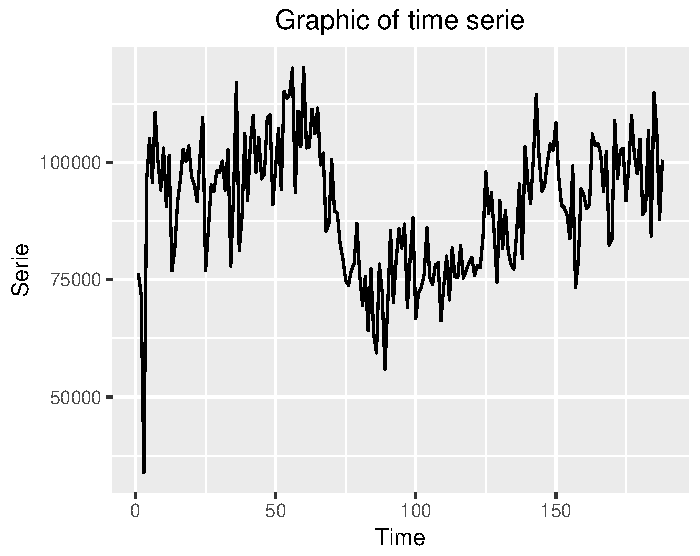
\includegraphics[width=\columnwidth]{time_serie.pdf}
		\caption{Exemplo de gráfico produzido pela função time\underline{ }series.}
		\label{fig:time_serie.pdf}
	\end{center}
\end{figure}

\subsection{Função \textit{patternsOnGraph}}

Sendo capaz de plotar o gráfico da série e mostrar ao usuário todas as partes deste que um determinado padrão aparece, tal função pode ainda possui dois modos de retorno, de acordo com a opção escolhida anteriormente. Assim como a funcionalidade descrita anteriormente tal função ainda não possui similar para dados bidimensionais.\\

\textbf{Input: } Série temporal, dimensão, delay, o padrão escolhido (É utilizado o índice dos padrões impressos na saída da função \textit{histogram}) e a opção de retorno.

\textbf{Output: } De acordo com a opção de retorno, pode ter como saída:

\begin{itemize}
\item Option = 0
	\begin{itemize}
	\item Será mostrado apenas o primeiro ponto de cada réplica do padrão presente na série.
	\end{itemize}
\item Option != 0
	\begin{itemize}
	\item Serão mostrados todos os pontos das réplicas do padrão escolhido ao longo da série.
	\end{itemize}
\end{itemize}

\begin{lstlisting}
patternsOnGraph<-function(serie,dimension,delay,number_of_pattern,
point=0){
  serie=na.omit(serie)
  lengthW=0
  point_time=point_value=c(1:length(serie))
  p_patterns <- formationPattern(serie,dimension,delay)
  n_symbols <- formationPattern(serie,dimension,delay,1)
  symbols <- definePatterns(dimension)
  elements <- formationPattern(serie,dimension,delay,2)
  index <- formationPattern(serie,dimension,delay,3)
  for(i in 1:n_symbols){
    if(all(p_patterns[i,]==symbols[number_of_pattern,])){
      if(points==0){
        lengthW = lengthW + 1
        point_value[lengthW]=elements[i,1]
        point_time[lengthW]=index[i,1]
      }
      else{
        for(j in 1:dimension){
          lengthW=lengthW+1
          point_value[lengthW]=elements[i,j]
          point_time[lengthW]=index[i,j]
        }
      }
    }
  }
  if(lengthW!=0){
    qplot(x=c(1:length(serie)),y=serie,geom="line",xlab="Time",
   	  ylab="Serie") + ggtitle("Graphic of time serie") +
      theme(plot.title = element_text(hjust=0.5)) +
      geom_point(aes(x=point_time[1:lengthW],y=point_value[1:lengthW]),
      color="blue")
  }else{
    qplot(x=c(1:length(serie)),y=serie,geom="line",xlab="Time",
    ylab="Serie") + ggtitle("Graphic of time serie") +
    theme(plot.title = element_text(hjust=0.5))
  }
}
\end{lstlisting}

\begin{figure}[!hbt]
	\begin{center}
		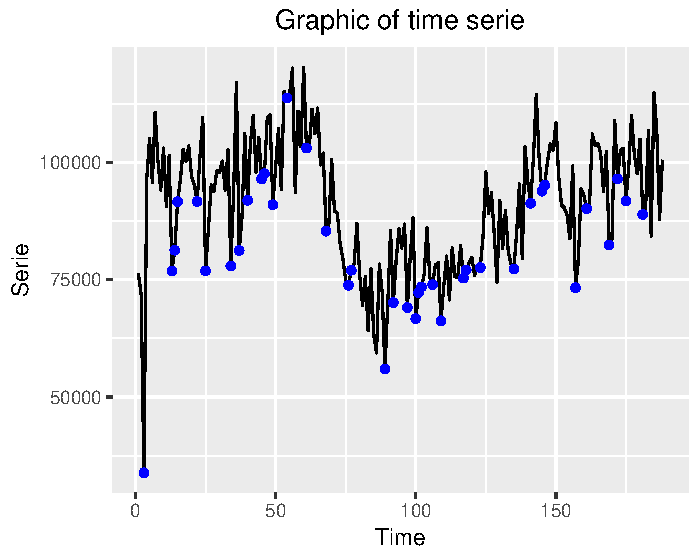
\includegraphics[width=\columnwidth]{patternOnGraph.pdf}
		\caption{Exemplo de gráfico produzido pela função patternsOnGraph, com number\underline{ }of\underline{ }pattern = 1 e points = 0}
		\label{fig:patternOnGraph.pdf}
	\end{center}
\end{figure}

\subsection{Função \textit{histogram}}

Tal função possui como retorno o histograma da frequência relativa dos padrões da série temporal, isto é, o histograma da distribuição de probabilidade, assim como também imprime tais padrões, para que o usuário esteja familiarizado sobre qual padrão apresentado no gráfico corresponde, uma vez que neste serão apresentados apenas os índices e não os padrões em si.\\

\textbf{Input: } Série temporal, dimensão e delay.

\textbf{Output: } Histograma da distribuição de probabilidade e será impresso os padrões.\\

\begin{lstlisting}
histogram<-function(serie,dimension,delay){
  fat=factorial(dimension)
  p_patterns <- formationPattern(serie,dimension,delay)
  n_symbols <- formationPattern(serie,dimension,delay,1)
  symbol <- definePatterns(dimension)
  index_rep=array(0,n_symbols)
  for(i in 1:n_symbols){
    for(j in 1:fat){
      if(all(p_patterns[i,]==symbol[j, ])){
        index_rep[i]=j
        break
      }
    }
  }
  index_rep=index_rep[1:n_symbols]
  p = qplot(index_rep,geom="histogram",xlab="Patterns",ylab="Density",
  	binwidth=1) + ggtitle("Histogram of the patterns") +
    theme(plot.title = element_text(hjust=0.5))
  plot(p)
  print(symbol)
}
\end{lstlisting}

\begin{figure}[!hbt]
	\begin{center}
		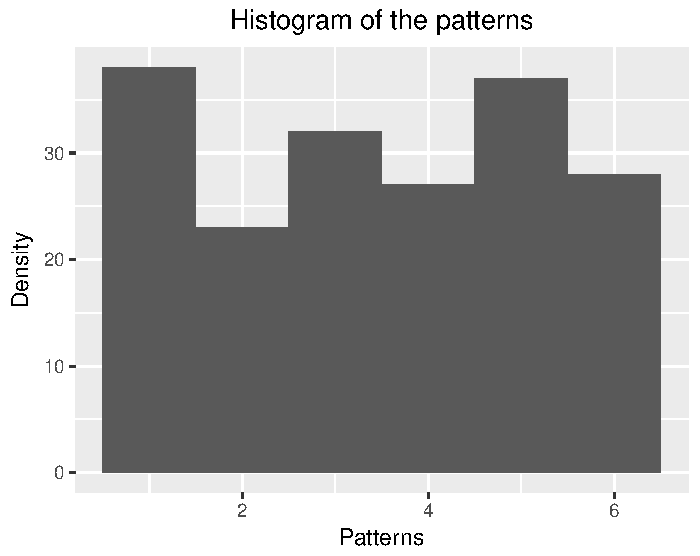
\includegraphics[width=\columnwidth]{histogram.pdf}
		\caption{Exemplo de gráfico produzido pela função histogram}
		\label{fig:histogram.pdf}
	\end{center}
\end{figure}

\subsection{Função \textit{histogramImage}}

Semelhante a função \textit{histogram} descrita anteriormente, tal funcionalidade possui as mesmas características desta, possuindo apenas como diferencial que a última demonstra o histograma da distribuição de probabilidade de dados bidimensionais.\\

\textbf{Input: } Imagem a ser analisada, dimensões x e y, delays x e y e a dimensão total da imagem (esta possui como padrão o valor 0, que representa que deverá ser analisada a dimensão original da imagem).

\textbf{Output: } Histograma da distribuição de probabilidade e será impresso os padrões.\\ 

\begin{lstlisting}
histogramImage<-function(myImg,dimx,dimy,delx,dely,dimension=0){  
  if(!dimension){
    dimension=dim(myImg)[1]
  }
  d = dimX*dimY
  fat = factorial(d)
  p_patterns = formationPatternsImage(myImg,dimX,dimY,delX,
  			   delY,dimension)
  n_symbols = formationPatternsImage(myImg,dimX,dimY,delX,
  			  delY,dimension, 1)
  symbols <- definePatterns(d)
  index_rep=array(0,n_symbols)
  for(i in 1:n_symbols){
    for(j in 1:fat){
      if(all(p_patterns[i,]==symbols[j, ])){
        index_rep[i]=j
        break
      }
    }
  }
  index_rep=index_rep[1:n_symbols]
  p = qplot(index_rep,geom="histogram",xlab="Patterns",ylab="Density",
  	  binwidth=1) + ggtitle("Histogram of the patterns") +
      theme(plot.title = element_text(hjust=0.5))
  plot(p)
  print(symbols)
}
\end{lstlisting}

\section{Distâncias estocásticas}

Funções presentes no arquivo \textbf{\textit{Distances.R}}.\\

\textbf{Input: } Distribuição de probabilidade da série a ser estudada.

\textbf{Output: } Valor da distância referente a função.\\ 

\begin{lstlisting}

euclidian_distance<-function(probability){
  c = rep(1/length(probability),length(probability))
  distance = sum((probability-c)^2)
  return(sqrt(distance))
}

euclidian_quadratica_distance<-function(probability){
  c = rep(1/length(probability),length(probability))
  distance = sum((probability-c)^2)
  return(distance)
}

manhattan_distance<-function(probability){
  c = rep(1/length(probability),length(probability))
  distance = sum(abs(probability-c))
  return(distance)
}

chebyshev_distance<-function(probability){
  c = rep(1/length(probability),length(probability))
  L = abs(probability - c)
  return(max(L))
}

kullback_leibler_divergence<-function(probability){
  c = rep(1/length(probability),length(probability))
  distance <- probability * log(probability/c)
  distance[is.nan(distance)] <- 0
  return(sum(distance))
}

kullbach_aux<-function(p,q){
  distance <- p * log(p/q)
  distance[is.nan(distance)||is.infinite(distance)]<-0
  return(sum(distance))
}

hellinger_Distance<-function(probability){
  c = rep(1/length(probability),length(probability))
  distance = sum((sqrt(probability)-sqrt(c))^2)*0.5
  return(sqrt(distance))
}

jensenDivergence<-function(p){
  q = rep(1/length(p),length(p))
  s_p = shannonEntropy(p)
  s_q = shannonEntropy(q)
  s_pq = shannonEntropy((p+q)/2)
  divergence = sum( s_pq - (s_p/2) - (s_q/2))
  return(divergence)
}

constant <- function(p){
  v1 = (0.5)/length(p)
  aux1 = (0.5 + v1) * log(0.5 + v1)
  aux2 = (length(p) - 1) * v1 * log(v1)
  aux3 = (1 - 0.5) * log(length(p))
  q03 = -1/(aux1 + aux2 + aux3)
  return(q03)
}

C<-function(p){
  c <- jensenDivergence(p) * constant(p) *
  		shannonEntropyNormalized(p)
  return(c)
}

wootters_distance<-function(probability,q){
  c = rep(1/length(probability),length(probability))
  dis = sum(sqrt(probability*c))
  dis = acos(dis)
  return(dis)
}

complexityF<-function(probability){
  entropy = ShannonAux(probability)
  qInitial = rep(1/length(probability),length(probability))
  qInitial[1] = 1
  desequilibrium = jensenDivergence(qInitial) *
  					jensenDivergence(probability)
  comp = entropy * desequilibrium
  return(comp)
}
\end{lstlisting}

\section{Entropias}

Funções presentes no arquivo \textbf{\textit{Entropys.R}}.\\

\textbf{Input: } Distribuição de probabilidade da série a ser estudada, a opção de retorno e em algumas é necessário informar a variável \textit{q}.

\textbf{Output: } De acordo com a opção de retorno, podemos ter as seguintes saídas:

\begin{itemize}
\item Option = 1
	\begin{itemize}
	\item Retorna a entropia referente a função escolhida.
	\end{itemize}
\item Option != 1
	\begin{itemize}
	\item Retorna a entropia normalizada da função escolhida.
	\end{itemize}
\end{itemize}

\begin{lstlisting}

shannonEntropy <- function(probability){
  h <- probability * log(probability)
  h[is.nan(h)] <- 0
  return (-sum(h))
}

shannonEntropyNormalized <- function(probability){
  return(shannonEntropy(probability)/log(length(probability)))
}

tsallisEntropy <- function(probability,q,option=0){  
  entropy = sum(probability^q)
  entropy = (1 - entropy)*(1/(q - 1))
  if(option){
    return (entropy)
  }
  else{
    ent_max = (1 - (length(probability)^(1 - q)))/(q - 1)
    return( entropy/ent_max)
  }
}

renyiEntropy <- function(probability,q,option=0){
  entropy = sum(probability^q)
  entropy = log(entropy)
  entropy = entropy * (1/(1 - q))
  if(option){
    return (entropy)
  }
  else{
    return ( entropy/log(length(probability)))
  }
}
\end{lstlisting}

\section{Plano entropia-complexidade}

Funções presentes no arquivo \textbf{\textit{complexity-entropy.R}}.\\

\textbf{Observação:} Para a implementação de tais funcionalidades foi necessária a utilização do pacote \textit{\textbf{ggplot2}} da linguagem \textit{R}.

O processo de plotagem do plano entropia-complexidade é dado em duas partes: a primeira consiste na simples plotagem dos valores máximos e mínimos da curva e a segunda na plotagem dos reais valores de complexidade e entropia. Logo, como esperado foram implementadas duas funções para 
desempenhar tais atividades.

\subsection{Função \textit{readingMPR}}

\textbf{Observação: } Tal funcionalidade será apenas uma função auxiliar da \textit{partitionMPR}  e para utilizá-la é necessário que os arquivos contendo os dados utilizados nesta estejam no mesmo diretório.

\textbf{Input: } Dimensão e opção de retorno.

\textbf{Output: } De acordo com a opção de retorno pode oferecer como saída os valores x ou y das curvas que representam os valores máximos ou mínimos de complexidade.

\begin{lstlisting}

readingMPR<-function(dimension,option=0){
  if(dimension == 3){ 
    continua = "continuaN6.txt"
    trozo = "trozosN6.txt"
  }
  if(dimension == 4){ 
    continua = "continuaN24.txt"
    trozo = "trozosN24.txt"
  }
  if(dimension == 5){ 
    continua = "continuaN120.txt"
    trozo = "trozosN120.txt"
  }
  if(dimension == 6){ 
    continua = "continuaN720.txt"
    trozo = "trozosN720.txt"
  }
  curva1x = Read_txt2(continua,1) 
  if(option==1) return(curva1x)
  curva1y = Read_txt2(continua,2)
  if(option==2) return(curva1y)
  curva2x = Read_txt2(trozo,1)
  if(option==3) return(curva2x)
  curva2y = Read_txt2(trozo,2)
  if(option==4) return(curva2y)
}

\end{lstlisting}

\subsection{Função \textit{partitionMPR}}

Função responsável pela plotagem do plano, assim como também pelo cálculo dos valores de complexidade e entropia.

\textbf{Input: } Série, dimensão, delay e o número de partições que se deseja que a série seja particionada.

\textbf{Output: } Plotagem do plano e os valores de entropia e complexidade.

\begin{lstlisting}
partitionMPR<-function(series,dimension,delay,partition){
  complexity = entropy = rep(0,partition)
  div = floor(length(series)/partition)
  if(partition != 1){
    for(i in 1:partition){
      initial = ((i-1)*div)
      end = initial + div
      if(i == 1){
        initial = 1
        end = div
      }
      aux = series[initial:end]
      probability = distribution(aux,dimension,delay)
      entropy[i] = shannonEntropyNormalized(probability)
      complexity[i] = C(probability)
    }
  }
  else{
    probability = distribution(series,dimension,delay)
    entropy = shannonEntropyNormalized(probability)
    complexity = C(probability)
  }
  print(entropy)
  print(complexity)
  c1x = readingMPR(dimension,1)
  c1y = readingMPR(dimension,2)
  c2x = readingMPR(dimension,3)
  c2y = readingMPR(dimension,4)
  qplot(x=c2x,y=c2y,geom="line",xlab="Shannon Entropy",
  	ylab="MPR Statistical Complexity") +
    ggtitle("Plane Complexity Entropy") +
    theme(plot.title = element_text(hjust=0.5)) +
    geom_line(aes(x=c1x,c1y)) + 
    geom_point(aes(x=entropy,y=complexity),color="blue")
}
\end{lstlisting}

\begin{figure}[!hbt]
	\begin{center}
		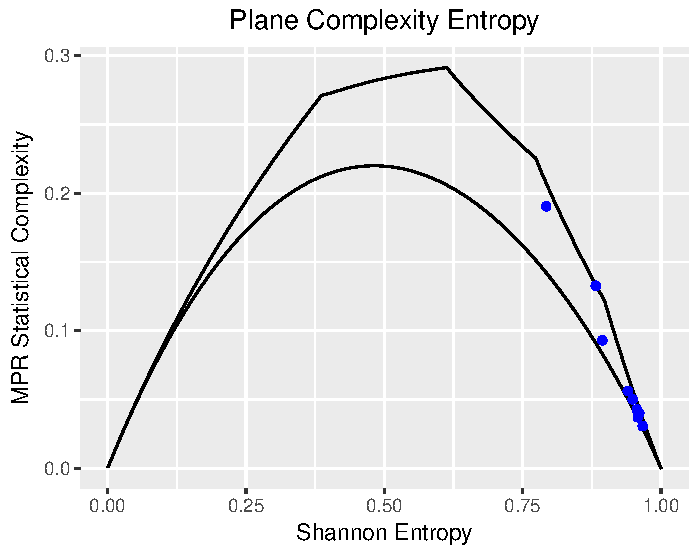
\includegraphics[width=\columnwidth]{complexity-entropy.pdf}
		\caption{Exemplo de Plano entropia-complexidade produzido pelas funções citadas acima, onde dimension = 3}
		\label{fig:complexity-entropy.pdf}
	\end{center}
\end{figure}

Tal funcionalidade ainda não possui semenlhante para dados bidimensionais, uma vez que não possuímos em mãos os valores das curvas máximas e mínimas.

\section{Funções de mineração de dados ou pré-processamento}

Tais funções já se encontram detalhadas no relatório \textit{Mineração de dados utilizando séries temporais} disponível no repositório do projeto no \textbf{GITHUB}.

\section{Conclusões}

Logo, foram detalhadas e explicadas minuciosamente o funcionamento de cada função implementada ao longo do projeto, sendo este então capaz de análise e possíveis testes, visando sempre a melhoria e crescimento de tal pesquisa.

\end{document}